%&pdflatex
%
%  Comparison of Numerical Models for Coastal Dynamics - 1D Theory
%
%  Authors:
%
\documentclass[]{article}

\usepackage{graphicx}

% Use utf-8 encoding for foreign characters
\usepackage[utf8]{inputenc}

% Multipart figures
% \usepackage{subcaption}

% More symbols
\usepackage{amsmath}
\usepackage{amssymb}
\usepackage{latexsym}

% URL and linking help
\usepackage{hyperref}

% Package for including code in the document
\usepackage{listings}
% \DeclareCaptionFont{white}{\color{white}}
% \DeclareCaptionFormat{listing}{%
%   \parbox{\textwidth}{\colorbox{gray}{\parbox{\textwidth}{#1#2#3}}\vskip-4pt}}
% \captionsetup[lstlisting]{format=listing,labelfont=white,textfont=white}
% \lstset{frame=lrb,xleftmargin=\fboxsep,xrightmargin=-\fboxsep,numbers=left,basicstyle=\ttfamily\small,language=python,columns=fixed,commentstyle=\em\color[rgb]{0.133,0.545,0.133}}

% This is now the recommended way for checking for PDFLaTeX:
\usepackage{ifpdf}

% Add line numbers
\usepackage[mathlines]{lineno}

% Need to use this package to handle the spacing issues in LaTeX after a command
\usepackage{xspace}

% Markup
\usepackage{color}
\newcommand{\comment}[1]{\color{blue} #1}
\newcommand{\alert}[1]{\textbf{\color{red} #1}}

\graphicspath{{./figures/}}
% tables
\usepackage{booktabs}


% Useful commands
%!TEX root = paper.tex
%  Generic math macros
\renewcommand{\v}[1]{\boldsymbol{#1}}
\newcommand{\m}[1]{\text{\textsf#1}}

\newcommand{\pd}[2]{\ensuremath{\frac{\partial #1}{\partial #2}}} % partial
\newcommand{\dee}{\ensuremath{\mathrm{d}}}                  % d symbol
\newcommand{\diff}[2]{\ensuremath{\frac{\dee #1}{\dee #2}}} % Derivative d/dx
% \newcommand{\grad}{\ensuremath{\nabla}}                     % Gradient symbol
\newcommand{\gradient}{\ensuremath{\textsf{grad}}}          % Written gradient
\newcommand{\Div}{\ensuremath{\nabla \cdot}}                % Divergence
\newcommand{\divergence}{\ensuremath{\textsf{div}}}         % Written div
\newcommand{\del}{\ensuremath{\nabla}}                      % Same as gradient
\newcommand{\delsq}{\ensuremath{\nabla^2}}                  % Laplacian
\newcommand{\lap}{\ensuremath{\delsq}}                      % Laplacian
\newcommand{\dx}{\ensuremath{\Delta x}}                     % Delta x
\newcommand{\dy}{\ensuremath{\Delta y}}                     % Delta y
\newcommand{\dt}{\ensuremath{\Delta t}}                     % Delta t
\newcommand{\scinot}[2]{\ensuremath{#1\times10^{#2}}}       % Scientific note
\newcommand{\bigO}[1]{\ensuremath{\mathcal{O}(#1)}}         % Big O notation
\newcommand{\R}{\ensuremath{\mathbb{R}}}                    % Real field
\newcommand{\Z}{\ensuremath{\mathbb{Z}}}                    % Integer field
\newcommand{\half}{\ensuremath{\frac{1}{2}}}                % 1/2 fraction

%  Special formatting for codes
\newcommand{\geoclaw}{{\sc GeoClaw}\xspace}
\newcommand{\clawpack}{{\sc Clawpack}\xspace}
\newcommand{\amrclaw}{{\sc AMRClaw}\xspace}
\newcommand{\pyclaw}{{\sc PyClaw}\xspace}
\newcommand{\forestclaw}{Forestclaw\xspace}

%  Finite volume method symbols
\newcommand{\wave}{\ensuremath{\mathcal{W}}\xspace}             % Wave
\newcommand{\fwave}{\ensuremath{\mathcal{Z}}\xspace}            % F-Waves
\newcommand{\cell}{\ensuremath{\mathcal{C}}\xspace}             % FV grid cell
\newcommand{\apdq}{\ensuremath{\mathcal{A}^+ \Delta Q}\xspace}      % A+dq
\newcommand{\amdq}{\ensuremath{\mathcal{A}^- \Delta Q}\xspace}      % A-dq
\newcommand{\apmdq}{\ensuremath{\mathcal{A}^{\pm} \Delta Q}\xspace} % A+-dq

% B+-A+-dq symbols
\newcommand{\BpApdq}{\ensuremath{\mathcal{B}^{+} \mathcal{A}^{+} \Delta Q}\xspace}
\newcommand{\BpAmdq}{\ensuremath{\mathcal{B}^{+} \mathcal{A}^{-} \Delta Q}\xspace}
\newcommand{\BmApdq}{\ensuremath{\mathcal{B}^{-} \mathcal{A}^{+} \Delta Q}\xspace}
\newcommand{\BmAmdq}{\ensuremath{\mathcal{B}^{-} \mathcal{A}^{-} \Delta Q}\xspace}
\newcommand{\BpmApmdq}{\ensuremath{\mathcal{B}^{\pm} \mathcal{A}^{\pm} \Delta Q}\xspace}

% commands for nonhydrostatic part
\newcommand\Bt{Boussinesq-type}
\newcommand\Bte{\Bt\ equations}
\newcommand\da{depth-averaged}
\newcommand\nh{nonhydrostatic}
\newcommand\Nh{Nonhydrostatic}
\newcommand\nheswe{\nh\ extension for shallow water equations}
\newcommand\danheswe{\da\ \nheswe}
\newcommand\nhp{\nh\ pressure}
\newcommand\fnh{f_{\text{nh}}}
\newcommand\fgn{f_{\text{d}}}
\newcommand\bu{\boldsymbol{u}}
\newcommand\bU{\boldsymbol{U}}
\newcommand\bx{\boldsymbol{x}}
\newcommand\csw{c_{\text{sw}}}
\newcommand\Pnh{P^{nh}}
\newcommand\Pnhd{P^{nh}_{-d}}
\newcommand\pnh{p^{nh}}
\newcommand\bnabla{\boldsymbol{\nabla}}




\begin{document}

\ifpdf
\DeclareGraphicsExtensions{.pdf, .png, .jpg, .tif}
\else
\DeclareGraphicsExtensions{.png, .jpg, .tif, .eps}
\fi

\title{Comparison of Numerical Models for Coastal Dynamics}

\author{Kyle T. Mandli\thanks{
            Columbia University} \and
        Nishant Panda\thanks{
            Colorado State University} \and
        Anja Jeschke\thanks{
            University of Hamburg}
        }

\maketitle

\begin{abstract}
    Put really awesome abstract here.
\end{abstract}

\begin{itemize}
    \item Theoretical Paper
    \begin{enumerate}
        \item Intro to different PDE systems being considered
        \item Dispersion analysis
        \item 1D tests
        \item status
        \begin{enumerate}
            \item KdV (Panda)
            \item Serre-Green-Naghdi (Panda)
            \item Boussinesq-Green-Naghdi (Panda)
            \item Shallow water (Mandli)
            \item 2-layer shallow water (Mandli)
            \item Nonhydrostatic extension for shallow water equations (Jeschke)
        \end{enumerate}
    \end{enumerate}
\end{itemize}



\begin{tabular}{c|ccccc}
\textbf{Model} & Well-balanced & Inundation & 2D & Non-Hydrostatic & Linear Dispersion \\
\hline \hline
SWE                     & yes & yes & yes &  no &  ~  \\
Serre-Green-Naghdi      &  ~  &  ~  &  ~  &  ~  &  ~  \\
Boussinesq-Green-Naghdi &  ~  &  ~  &  ~  &  ~  &  ~  \\
Non-Linear KdV          &  ~  &  ~  &  ~  &  ~  &  ~  \\
2-Layer SWE             & yes & yes & yes &  no &  ~  \\
Non-hydrostatic         & yes & ca. & yes & yes &  ~  \\
\end{tabular}

\section{Introduction}

\subsection{Selection Criteria}
\begin{itemize}
    \item Limit models to those that have the following properties:
    \begin{itemize}
        \item Well-balanced
        \item Handles inundation?
        \item 2D or at the most semi-3D (layers) - this may troublesome to differentiate as most hydrostatic ocean codes are really layered 3D models
    \end{itemize}
\end{itemize}

\section{Models} 
need to define same symbols for all models
%!TEX root = paper.tex
\subsection{Depth-averaged \nheswe}
The \nheswe\ is linked to the solution of the Euler equations using kinematic boundary conditions on the surface and the bottom. The basis of the method is a projection method (see e.g. \cite{Chorin.1968}) solving the time-discretized equations stepwise. 
The pressure is decomposed into a hydrostatic and a \nh\ part \cite{CasulliStelling.1998, StansbyZhou.1998}. This splitting has the advantage that the solver for the \nh\ equations can resort to the solver for the shallow water equations. 
The \da\ version of this apporach was derived from a multi-layer formulation  \cite{StellingZijlema.2003} applying linear approximations between different layers, s.t. also the \nhp\ is assumed to be linear in the multi-layer equations. On the other hand, the vertical Euler equation leads to a quadratic vertical profile of the \nhp when considering \da\ equations. Therefore, there are two possibilities to choose the pressure profile.
Under the assumption of small vertical variations of horizontal velocities, the \danheswe\ is derived out of the Euler equations for \da\ variables
\begin{align}
  (u,v)=\bu:=\frac{1}{h}\int_{-d}^{\xi}{\bU}\,dz, \qquad w:=\frac{1}{h}\int_{-d}^{\xi}{W}\,dz, \qquad \pnh&:=\frac{1}{h}\int_{-d}^{\xi}{\Pnh}\,dz. \label{eq:def_pnh}
\end{align}
The \danheswe\ is described with the equation system
\begin{align}
\partial_t \xi+\bnabla \cdot (h\bu)=&0, \label{eq:nh_conti} \\
\partial_t \bu+(\bu \cdot \bnabla)\bu=&-g\bnabla \xi-\frac{1}{\rho h}\left(\bnabla \left(hp^{nh} \right) -\fnh\pnh \bnabla d\right), \label{eq:nh_Momxy} \\
\partial_t w+(\bu \cdot \bnabla)w=&\frac{1}{\rho h}\fnh\pnh, \label{eq:nh_Momz} \\
2 \left(w+\bu \cdot \bnabla d \right)=&-h\left(\bnabla \cdot \bu\right), \label{eq:nh_closure}
\end{align} 
where the scalar $\fnh$ refers to the chosen pressure profile. In case of the linear pressure profile
\begin{equation}
  P^{nh}(z)=\frac{\Pnhd}{h}(\xi -z),
\end{equation}
with $\Pnhd$ being the \nhp\ at the bottom, it is $\fnh=2$, whereas it is $\fnh=1.5$ in the case of the quadratic pressure profile
\begin{equation}
 P^{nh}(z)=\frac{1}{2}\frac{\Gamma}{h}\left(-(z+d)^2+h^2\right)%+\rho\Phi\left(\xi-z\right) \label{eq:Pnh_quadr_z}
\end{equation}
with
\begin{align*}
  \Gamma &:= \rho h\left( -(\bnabla \cdot \partial_t \bu) - (\bu \cdot \bnabla) (\bnabla \cdot \bu) + (\bnabla \cdot \bu)^2 \right). \\
  %\Phi &:= - \bnabla d \cdot \left( \partial_t  \bu + (\bu \cdot \bnabla)\bu \right) - \bu \cdot \bnabla(\bnabla d) \cdot \bu.
\end{align*}
For a more detailed derivation see \cite{Jeschke.2016}.


The spatial discretization of the shallow water equations implements the $P^{NC}_1$--$P_1$ finite element method as described in \cite{Hanert.2005, LeRouxPouliot.2008} with the $P^{NC}_1$--$P_1$ advection scheme of \cite{Androsov.2011}. It uses nonconforming linear basis functions for the horizontal velocities and conforming linear basis functions for the height. A two-dimensional computational domain is represented by a structured triangulation generated with the adaptive mesh generator amatos \cite{Behrens.2005}. The time-stepping scheme applies the Leapfrog method stabilized with the Robert-Asselin filter \cite{Asselin.1972} using $\alpha=0.025$.

The \danheswe\ \eqref{eq:nh_conti}--\eqref{eq:nh_Momz} is solved based on the projection method proposed in \cite{StellingZijlema.2003}. The advantage of this method is that the shallow water solver does not have to change in order to solve the \nh\ equation system. This projection method involves the solution of a Poisson equation for the \nhp\ in each timestep, which is constructed as follows: The time-discretized horizontal momentum equations are written as an intermediate solution in the present timestep plus a correction term depending on the \nhp. Together with the time-discretized vertical momentum equation, this splitting is substituted into equation \eqref{eq:nh_closure} in its weak formulation to receive the Poisson equation. The emerging linear equation system is solved by means of a GMRES algorithm. The computed \nhp\ is added to the intermediate horizontal velocities and to the vertical velocity of the previous time step. At this point, the velocities have been updated and the numerical solution of the continuity equation completes the computation of the timestep.
To discretize the \nhp\ and vertical velocity, conforming linear basis functions are used. The same approach was taken in \cite{Fuchs.2013}, but we retain an absent bathymetry gradient term. 

\section{Dispersion Analysis} \label{sec:dispersion}
For simplicity, we restrict ourselves to the linear one-dimensional case on a constant bathymetry.
We consider harmonic solutions 
\[
 \xi=\overline{\xi}e^{i(\kappa x-\omega t)}, \qquad u=\overline{u}e^{i(\kappa x-\omega t)},
\]
in each equation system with the wave number $\kappa$, the frequency $\omega$ and the time $t$ for given amplitudes $\overline{\xi}$ and $\overline{u}$.
%!TEX root = paper.tex
\subsection{Depth-averaged \nheswe}
The linearized system of equations \eqref{eq:nh_conti}--\eqref{eq:nh_closure} reduces to 
\begin{align*}
 0 &= \partial_t\xi+\partial_x(du), \\
 \partial_tu + g\partial_x\xi &= \frac{1}{2\fnh}d^2\partial_{txx} u,
%  \label{eq:nh_1D_Bouss_Disp}
\end{align*}
where the scalar $\fnh$ determines the vertical pressure profile. The resulting dispersion relation is
\begin{equation}
 \omega^2_{\text{nh,}\fnh}=\frac{\csw^2\kappa^2}{1+\frac{(\kappa d)^2}{2\fnh}},
 \label{eq:disp_nh_fnh}
\end{equation}
where $\csw=\sqrt{gd}$ is the linear shallow water gravity wave speed.
The dispersion relation resulting from the quadratic vertical pressure profile ($\fnh=\frac{3}{2}$) is the same as for the Serre equations, so
\begin{equation}
 \omega^2_{\text{nh,quad}}=\frac{\csw\kappa^2}{1+\frac{(\kappa d)^2}{3}}=\csw^2\kappa^2\left(1-\frac{1}{3}(kd)^2+\frac{1}{9}(kd)^4+\mathcal{O}(kd)^6 \right),
 \label{eq:disp_nh_quadr}
\end{equation}
whereas the linear vertical pressure profile ($\fnh=2$) leads to the dispersion relation
\begin{equation}
 \omega^2_{\text{nh,lin}}=\frac{\csw^2\kappa^2}{1+\frac{(\kappa d)^2}{4}}=\csw^2\kappa^2\left(1-\frac{1}{4}(kd)^2+\frac{1}{16}(kd)^4+\mathcal{O}(kd)^6 \right) \label{eq:disp_nh_lin}
\end{equation}
% The same result is given in \cite{Cui.2014} for the linear vertical profile.
For comparison, the dispersion relation from the full linear inviscid equations
is (see, for instance, \cite{Whitham.1974})
\begin{equation}
 \omega^2_{\text{full}}=g\kappa\tanh\left(\kappa d  \right)=\csw^2\kappa^2\left(1-\frac{1}{3}(kd)^2+\frac{2}{15}(kd)^4+\mathcal{O}(kd)^6 \right) .
 \label{eq:disp_full}
\end{equation}
Therefore, the quadratic vertical profile of the \nhp\ is exact in comparison with the dispersion relation from the full linear inviscid equations up to the first order, whereas the linear profile leads to a match only in the zeroth order.

\section{Benchmarks}

\begin{itemize}
    \item \url{https://github.com/rjleveque/nthmp-benchmark-problems}
    \item \url{https://github.com/rjleveque/geoclaw-group/tree/master/benchmarks}
    \item \url{https://github.com/rjleveque/tsunami_benchmarks}
    \item \url{http://depts.washington.edu/clawpack/geoclaw/benchmarks/nthmp_currents_2015/}
\end{itemize}

\begin{tabular}{c|cccc}
\textbf{Dimensionality} & \textbf{Benchmark} & Analytical & Experimental & Field \\
\hline \hline
1D & Solitary Wave on a Simple Beach    & X          & X & ~ \\
~  & Solitary Wave on a Composite Beach & X (linear) & X & ~ \\
~  & Solitary Wave translating          & X          & X & ~ \\
~  & Trapezoidal Berm                   & ~          & X & ~ \\
\end{tabular}

\subsection{Linear standing wave}
The linear standing wave test illustrates the different linear dispersion relations and the ability of the numerical method to represent them in an accurate manner. 
Both, the linearized systems of the hydrostatic and dispersive have an analytic standing wave solution
\begin{align}
\xi(\bx,t)&=-a\sin\left(\kappa x \right)\cos\left(\kappa ct\right), \\
 u(\bx,t) &=a \frac{c}{d}\cos\left(\kappa x\right)\sin\left(\kappa ct\right), \\
 v(\bx,t) &=0, \qquad \forall \ \bx=(x, y)^T \in \Omega, \forall t \in \mathbb{R},
\end{align}
where the phase velocity $c=\frac{\omega_{\text{nh,}\fnh}}{\kappa}$ is chosen for the dispersive equation set and $c=\csw$ for the hydrostatic equation set, respectively. For the \nh\ model, the analytic vertical velocity has to be defined as
\[
w(\bx,t)=-\frac{d}{2}\partial_x u=\frac{1}{2}ac\kappa\sin\left(\kappa x \right)\sin\left(\kappa ct\right),
\]
which is derived directly from \eqref{eq:nh_closure}.
In different model runs, we vary the depth $d$ while keeping the wave length $\lambda=\frac{2\pi}{\kappa}=20$ m and the amplitude $a=0.01$m constant to get ratios for $\frac{d}{\lambda}$ between $0.05$ and $1.0$, and ratios for $\frac{a}{d}$ between $0.01$ and $0.005$, respectively.
We impose double periodic boundary conditions on a grid length of one wave length. The simulation time is chosen long enough to measure one wave period. 

\subsubsection{Results of \nh\ model}
The resulting normalized phase velocities for the shallow water model and the \nh\ equation set with either the linear or the quadratic vertical pressure are displayed in figure \ref{fig:nh_standingwave}. Furthermore, they are compared to their analytical reference phase velocities and the full reference phase velocity as derived in section \ref{sec:dispersion}. 
In each case, the numerical dispersion relation matches the corresponding analytical one precisely.
% The coincidence between numerical and analytical phase velocities is very good. 
In a close neighborhood of the shallow water assumption (i.e., in the limit $\frac{d}{\lambda} \rightarrow 0$), the quadratic vertical pressure profile gives a better phase velocity compared to the full reference solution than the linear profile, as expected from series expansions around this state used in \Bt\ models.
% \svnote{Can we have an additional detail plot of this neighborhood?} \ajnote{Then only thinner lines would help. I could also provide the whole image with different plotting style (thinner lines and ) One could also use absolute errors between numerical values and reference phase velocities. }\jbnote{What are you expecting to see?}\svnote{I expect to see what we describe in the text, i.e., that the quadratic vertical pressure profile gives a better phase velocity than the linear one near $d/\lambda=0$, see added figure.}
However, for ratios $\frac{d}{\lambda} > 0.25$ approximately, the linear profile matches better.

\begin{figure}[htbp]
        \includegraphics*[width=0.95\textwidth]{nh_standingwave.eps}
        \caption{Standing wave: Comparison of simulated hydrostatic and \nh\ phase velocities with analytic reference values for all simulations (left) and a zoom onto the close neighborhood of the long wave limit (right)}
        \label{fig:nh_standingwave}
\end{figure}


\subsection{Propagating solitary wave}
The propagating solitary wave tests the balancing of dispersion effects and nonlinearity for an appropriate initial condition.
On constant bathymetry, the Serre equations \cite{Serre.1953} have an analytic solitary wave solution
\begin{align}
\label{eq:Serre_sol_surface}
\xi(\bx,t)&=a \ \text{cosh}^{-2}(K(x-ct-x_0)), \\
u(\bx,t)&=c\frac{\xi(\bx,t)}{d+\xi(\bx,t)},
\end{align}
with the ratio $\frac{a}{d}=0.2$, propagation velocity $c=\sqrt{g(d+a)}$ on a constant depth $d=10 \, \text{m}$, scale factor $K=\sqrt{\left(\frac{3a}{4d^2(d+a)}\right)}$ and displacement $x_0=l/2$ on a domain of length $l=800 \, \text{m}$.
Again, we impose double periodic boundary conditions solitary wave propagating in the positive $x$-direction. The simulation time is $30$ seconds.

\subsubsection{Results of \nh\ model}
The equations \eqref{eq:nh_conti}--\eqref{eq:nh_closure} using the quadratic vertical pressure profile are equivalent to the Serre equations \cite{Serre.1953}, which is shown in  \cite{Jeschke.2016}. Using the linear vertical pressure profile, there is no equivalence to the Serre equations.
For the \nh\ model, we also need to initialize the vertical velocity, which directly follows from equation Equation \eqref{eq:nh_closure}, s.t.
\begin{align}
w&=-0.5h\partial_x u. \label{eq:nh_solit_init_w}
\end{align}
Figure \ref{fig:nh_solitarywave} compares our numerical computations with the analytical solution at the end of the simulation time.
The numerical result using the quadratic pressure profile shows a very good agreement with the analytical solution. In contrast, the application of the linear pressure profile yields a threefold mismatch arising from the inconsistency in initial conditions combined with the underlying equation system: Small amplitude waves propagate to the opposite direction, the wave height increases {because of weaker dispersion of the linear profile and trailing waves start to establish.
In \cite{StellingZijlema.2003, Walters.2005, Yamazaki.2008}, different solitary waves are computed with \nh\ models using the traditional linear vertical pressure profile. Therein, these mismatches are also visible, except that their amplitudes tend to diminish than to amplify. The reason is the application of another vertical velocity, namely $W(z)=-z\partial_x u$, so $w=-0.5(\xi-d)\partial_x u$. If the term $-d\partial_x u$ is added, the vertical velocity \eqref{eq:nh_solit_init_w} results. Hence, in \cite{StellingZijlema.2003, Walters.2005, Yamazaki.2008}, the vertical velocity is too large on the left hand side of the maximum amplitude and too small on the right hand side, which decreases the nonlinear steepening of the wave.
Their aim to compute the solitary waves was merely to show that \nh\ models produce similar results as \Bt\ models. 

\begin{figure}[htbp]
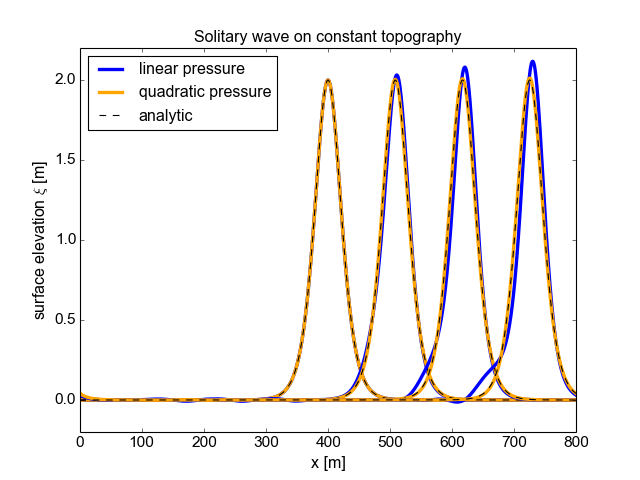
\includegraphics[width=\textwidth]{nh_solitary}
\caption{Comparison of the analytical (black) sea surface height of the
solitary wave with the simulation results of the quadratic (yellow) and linear (blue) vertical profile after a propagation time of 10, 20 and 30 seconds to the right.}
\label{fig:nh_solitarywave}
\end{figure}

%!TEX root = paper.tex
\subsection{Solitary wave on a composite beach} \label{sec:B_compositebeach}
This is an laboratory experiment conducted at the Coastal Engineering Laboratory of the U.S. Army Corps of Engineers and it is described in \url{http://nctr.pmel.noaa.gov/benchmark/Solitary_wave/}, \url{http://chl.erdc.usace.army.mil/chl.aspx?p=s&a=Projects;36}. 
A linear solitary (better called single) wave is propagating over a stepwise increasing bathymetry and it is reflected at a vertical wall on the right boundary. Different wave gauges measure the surface elevation and the runup on the vertical wall. 
The experimental data serve for validation of the models. Additionally to the experimental data, a linear analytic solution is provided, s.t. verification of our models is also tested.

Three different cases A, B, C with different target wave heights $a_t$, actual (measured) wave heights $a$ and distances $L$ of gauge $G4$ to the first step in the bathymetry at gauge $G5$. Table \ref{tab:compositebeach_cases} displays the three different cases and belonging data. We only consider case A at the moment. Measured runup data can be found in table \ref{tab:compositebeach_runup}, but are not compared yet to the simulations.

\begin{table}[htbp]
\begin{tabular}{lllll}
\textbf{Case} & \textbf{target $a_t / d$} & \textbf{actual $a / d$} & \textbf{dist. G4 to G5 [m]} & \textbf{dist. G4 to Wall [m]}  \\
\toprule
A       &     0.05   & 0.039    &   2.4   &  10.59     \\
B       &     0.30   & 0.264    &   0.89  &   9.17     \\
C       &     0.70   & 0.696    &    0.64  &   8.83    \\
\bottomrule
\end{tabular}
\caption{Data of three different cases}
\label{tab:compositebeach_cases}
\end{table}


\begin{table}[htbp]
\begin{tabular}{lll}
\textbf{Case} & \textbf{Runup R [cm]} & \textbf{R / d} \\
\toprule
A       &        2.74  &  0.13 \\
B       &       45.72  &  2.10 \\
C       &       27.43  &  1.26 \\
\bottomrule
\end{tabular}
\caption{Runup laboratory results of three different cases}
\label{tab:compositebeach_runup}
\end{table}


The initial condition is prescribed as 
\begin{itemize}
 \item a linear analytic solitary wave solution
\begin{align}
\xi(\bx,t)&=a_t \ \text{cosh}^{-2}(K(x-ct-x_0)), \\
u(\bx,t)&=c\frac{\xi(\bx,t)}{d},
\end{align}
with the initial target amplitude $a_t$, propagation velocity $c=\csw$ on a stepwise reduced depth starting from $d=0.218 \, \text{m}$ with scale factor $K=\sqrt{\left(\frac{3a_t}{4d^3}\right)}$ and displacement $x_0=10.59$, s.t. the initial solitary wave has its maximum at gauge G4 while the entire domain length is $L=24 \, \text{m}$. The simulation time is $20$ seconds. 
 \item the first option in \url{https://github.com/rjleveque/nthmp-benchmark-problems/blob/master/BP05-ElenaT-Solitary_wave_on_composite_beach_laboratory/BP5_description.pdf}. The velocities are set to zero and the doubled initial surface elevation $2\xi$ is prescribed at $x=0$. A doubled domain length of $L=48 \, \text{m}$ ensures that the waves reflected at the left boundary are not disturbing the solution. The simulation time is $40$ seconds.
\end{itemize}
We impose reflecting boundary conditions at the boundary in x-direction and periodic boundary conditions in y-direction. For the setup see figure \ref{fig:compositebeach_setup}. 
Because the analytic solution belongs to the linear SWE, corresponding models are expected to represent very good coincidence with this analytic solution.

\begin{figure}[htbp]
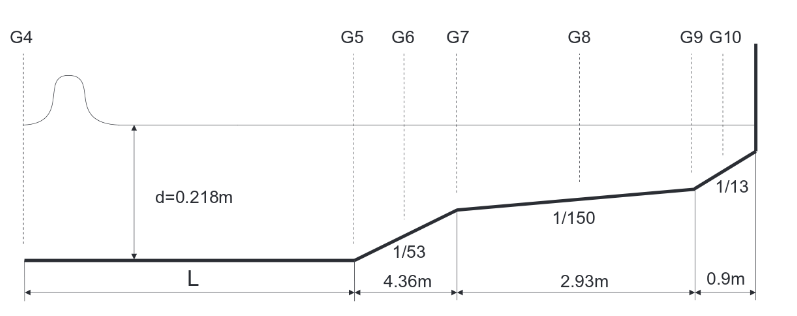
\includegraphics[width=\textwidth]{compositebeach_setup}
\caption{Setup of the testcase solitary wave on a composite beach}
\label{fig:compositebeach_setup}
\end{figure}

\subsubsection{Results of \nh\ model}
The results of the first and the seconds option are shifted by 271.5s to match the initial wave at gauge G4. Both are also scaled with a factor of $\frac{0.037}{0.05}$. % because $0.037$m seems to be the actual amplitude instead of $0.039$.
No difference between both options is visible in the figures then. Hence, we only plot the results of the (cheaper) first option using the linear SWE model and also the following results obtained with the \nh\ model.

Figures \eqref{fig:nh_compositebeach_ana_nh_Lhy} and \eqref{fig:nh_compositebeach_lab_nh_Lhy} display the comparison of the linear SWE with the linear analytic solution and experimental data, respectively.
The models results compared to the analytic solution are very good, while at gauges G9 and G10 a mismatch is visible, because the nonlinear regime is entered here (d $\in [0.047,0.117]$m, $a\approx0.008$m), for which the linear model is not suited.
The comparison to the experimental data reveals less dispersion and reduced amplitudes, although the overall match is also satisfactory.

Figures \eqref{fig:nh_compositebeach_ana_nh_Nnh12} and \eqref{fig:nh_compositebeach_lab_nh_Nnh12} display the comparison of the \nh\ equations using both the linear and the quadratic pressure profile with the linear analytic solution and experimental data, respectively. The \nh\ wave profile represents well the amplitudes, the shape of the propagating wave, the propagation velocities and also the developed dispersive wave train after reflecting of the laboratory surface elevation. The agreement with the linear analytic solution is worse, but still okay.
When wave hits step, the numerical sea surface height is not as much increased as the amplitude of exp data. 

Differences between both vertical pressure profiles are small, because dispersive effects become more significant after longer simulation time. However, the tendency of the linear profile to overestimate amplitudes, which was also visible in figure \ref{fig:nh_solitarywave}, is confirmed here, too. Additionally, we see that is also true not only for global maxima, but also for local maxima.

The analytic solution is a good test for the verification of the linear SWE model, whereas the laboratory data show its limits of applicability as well as that the dispersive model gives a more accurate physical representation of the experimental data.

Need to do: wq refl b.c. may be not good enough (not explicit treatment at the moment), edge integrals are missing.


\begin{figure}[htbp]
\begin{minipage}{\textwidth}
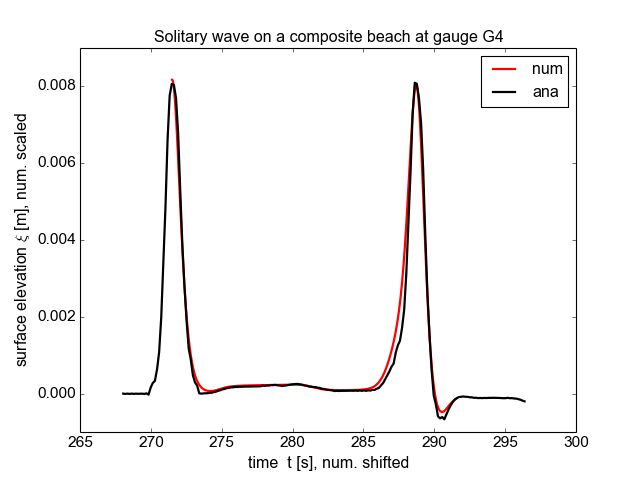
\includegraphics[width=0.48\textwidth]{compositebeach_ana_G4_nh_Lhy}
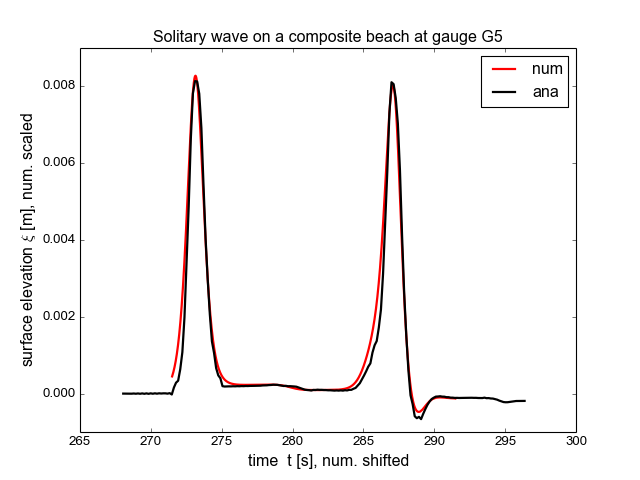
\includegraphics[width=0.48\textwidth]{compositebeach_ana_G5_nh_Lhy}
\end{minipage} \\
\begin{minipage}{\textwidth}
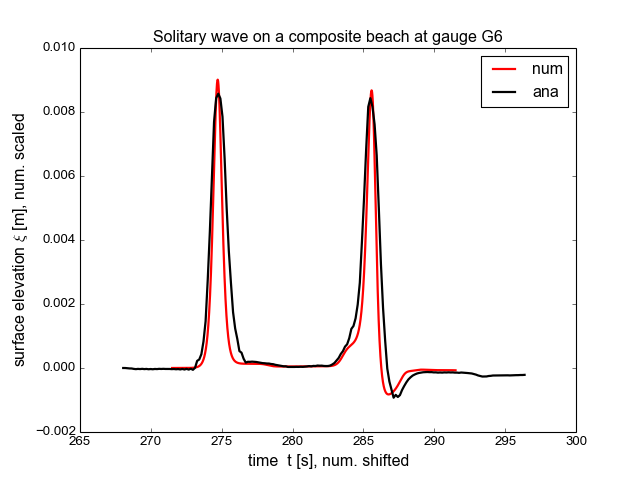
\includegraphics[width=0.48\textwidth]{compositebeach_ana_G6_nh_Lhy}
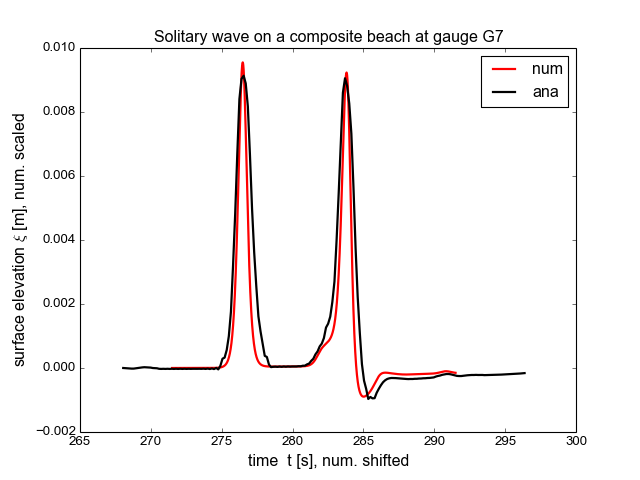
\includegraphics[width=0.48\textwidth]{compositebeach_ana_G7_nh_Lhy}
\end{minipage} \\
\begin{minipage}{\textwidth}
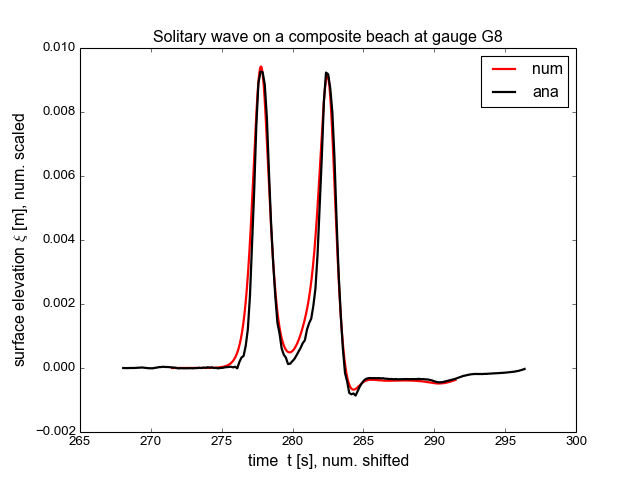
\includegraphics[width=0.48\textwidth]{compositebeach_ana_G8_nh_Lhy}
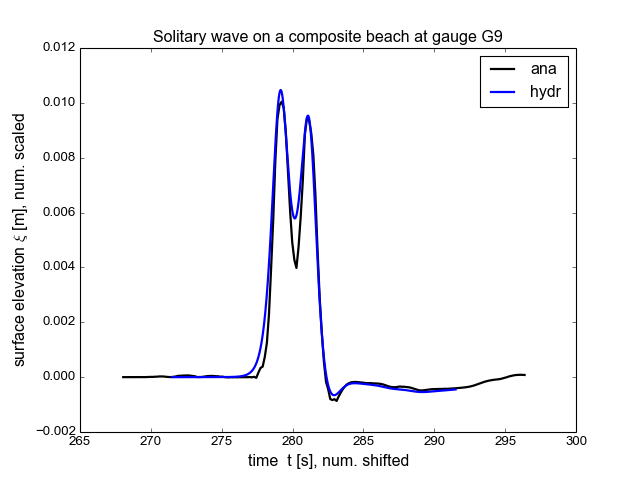
\includegraphics[width=0.48\textwidth]{compositebeach_ana_G9_nh_Lhy}
\end{minipage} \\
\begin{minipage}{\textwidth}
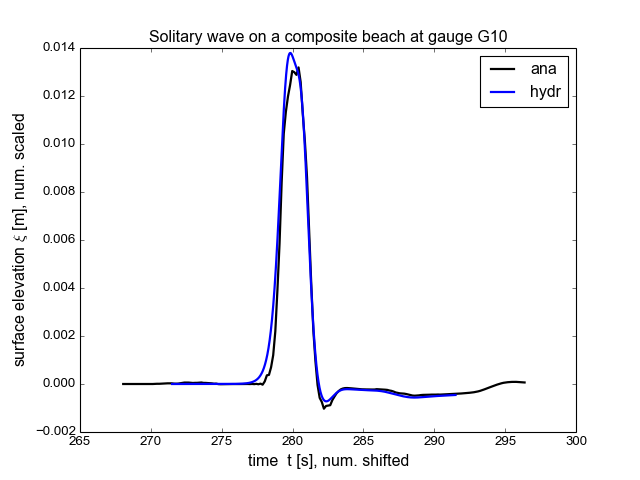
\includegraphics[width=0.48\textwidth]{compositebeach_ana_G10_nh_Lhy}
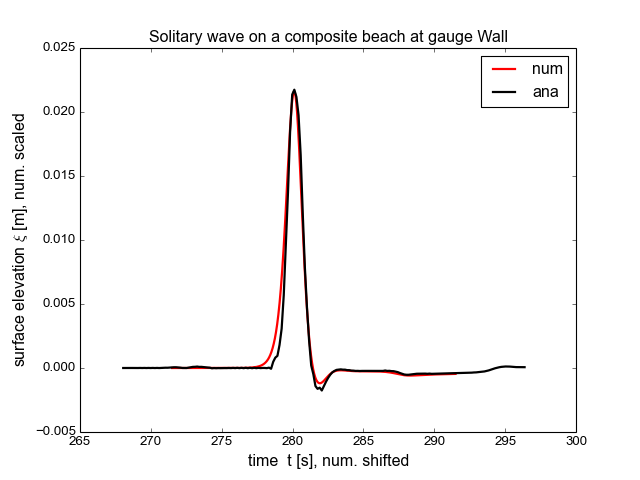
\includegraphics[width=0.48\textwidth]{compositebeach_ana_Wall_nh_Lhy}
\end{minipage}
\caption{Comparison of the analytical (black) sea surface height of the
solitary wave with the simulation results of the \nh\ model in its version of linear shallow water equations (blue)}
\label{fig:nh_compositebeach_ana_nh_Lhy}
\end{figure}

\begin{figure}[htbp]
\begin{minipage}{\textwidth}
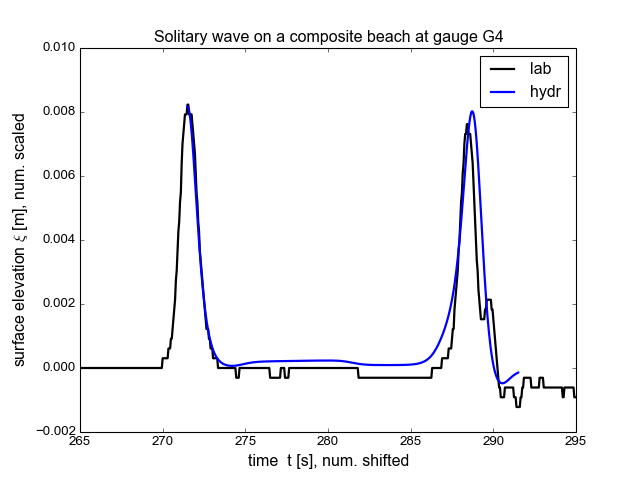
\includegraphics[width=0.48\textwidth]{compositebeach_lab_G4_nh_Lhy}
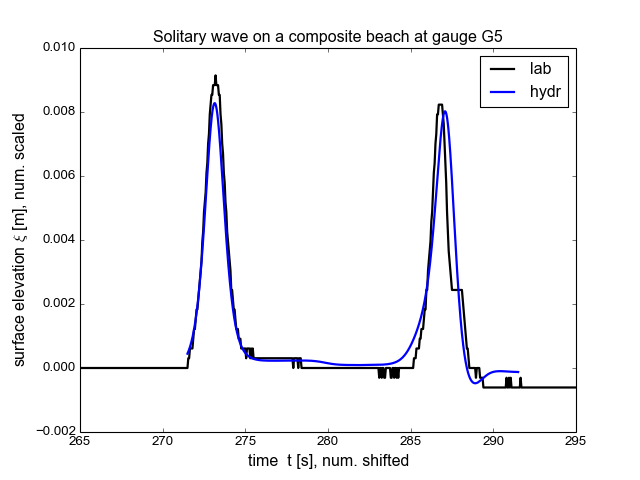
\includegraphics[width=0.48\textwidth]{compositebeach_lab_G5_nh_Lhy}
\end{minipage} \\
\begin{minipage}{\textwidth}
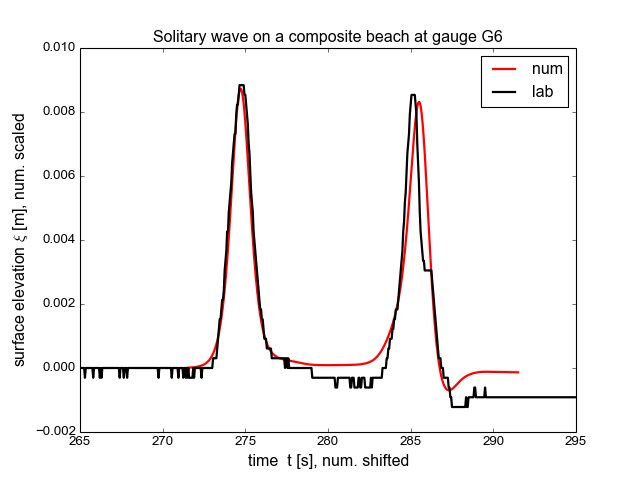
\includegraphics[width=0.48\textwidth]{compositebeach_lab_G6_nh_Lhy}
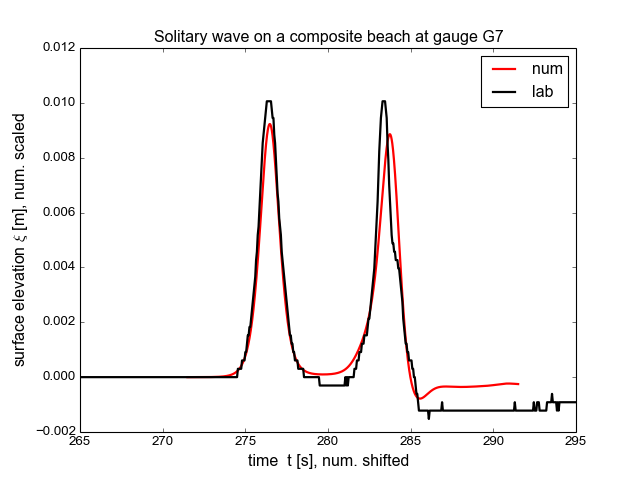
\includegraphics[width=0.48\textwidth]{compositebeach_lab_G7_nh_Lhy}
\end{minipage} \\
\begin{minipage}{\textwidth}
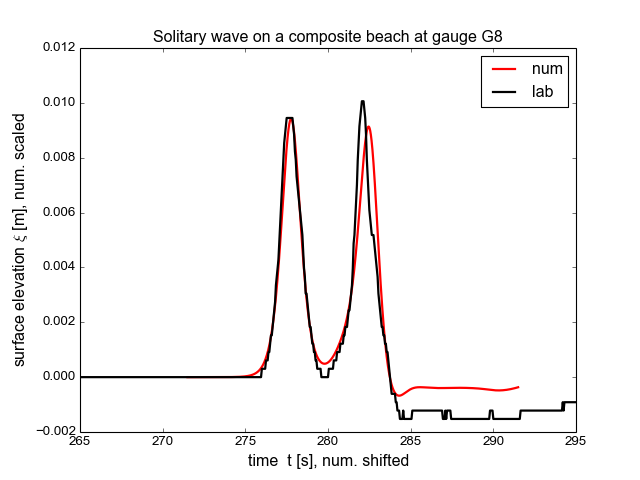
\includegraphics[width=0.48\textwidth]{compositebeach_lab_G8_nh_Lhy}
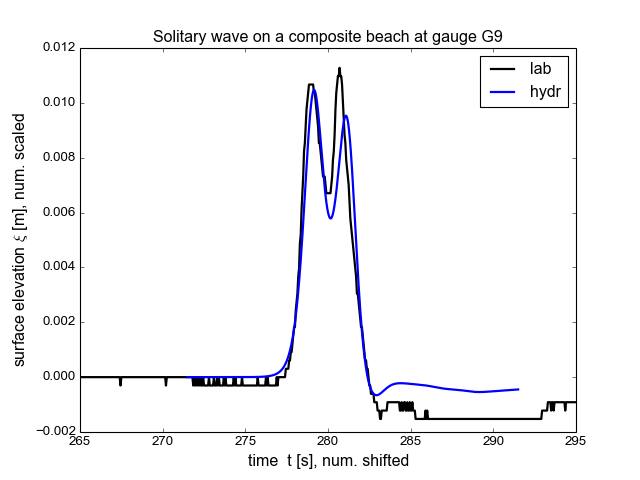
\includegraphics[width=0.48\textwidth]{compositebeach_lab_G9_nh_Lhy}
\end{minipage} \\
\begin{minipage}{0.48\textwidth}
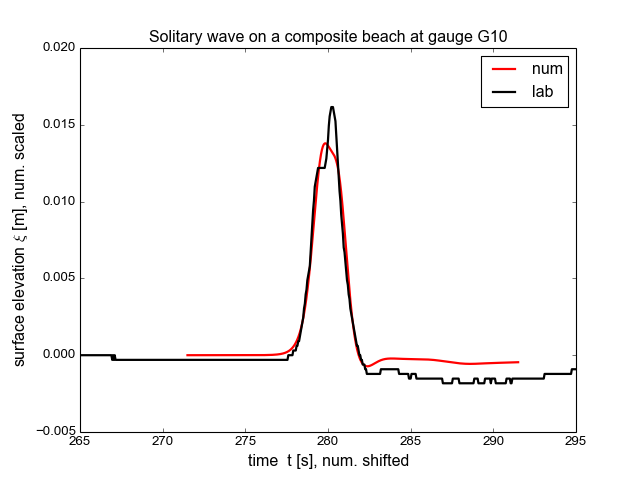
\includegraphics[width=\textwidth]{compositebeach_lab_G10_nh_Lhy}
\end{minipage} 
\begin{minipage}{0.45\textwidth}
\begin{tabular}{lll}
\textbf{Data} & \textbf{Runup} & \textbf{R / d} \\
              & \textbf{R [cm]} &  \\
\toprule
Exp.  &  2.74   &  0.13 \\
Model hydr. &  2.13   &  0.0978 \\
\end{tabular}
\end{minipage}
\caption{Comparison of the experimental (black) sea surface height of the
solitary wave with the simulation results of the \nh\ model in its version of linear shallow water equations (blue). The model runup is also scaled with 0.75.}
\label{fig:nh_compositebeach_lab_nh_Lhy}
\end{figure}



\begin{figure}[htbp]
\begin{minipage}{\textwidth}
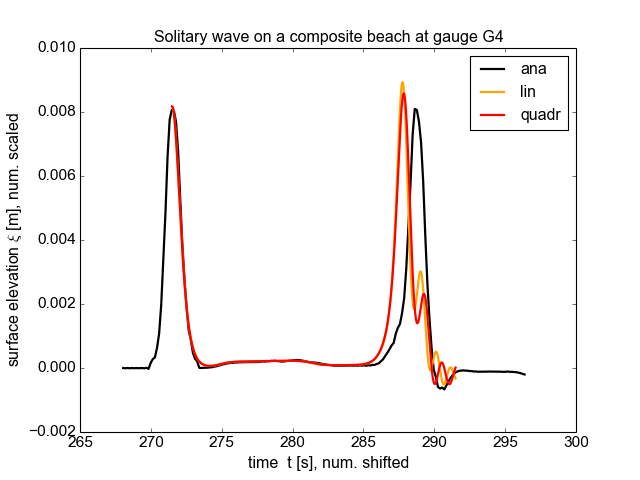
\includegraphics[width=0.48\textwidth]{compositebeach_ana_G4_nh_Nnh12}
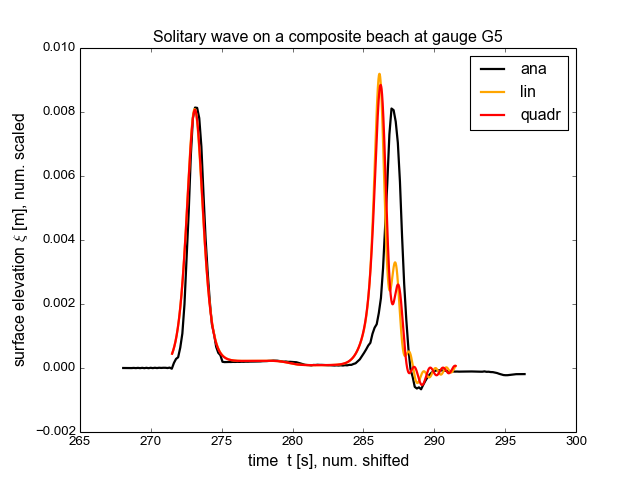
\includegraphics[width=0.48\textwidth]{compositebeach_ana_G5_nh_Nnh12}
\end{minipage} \\
\begin{minipage}{\textwidth}
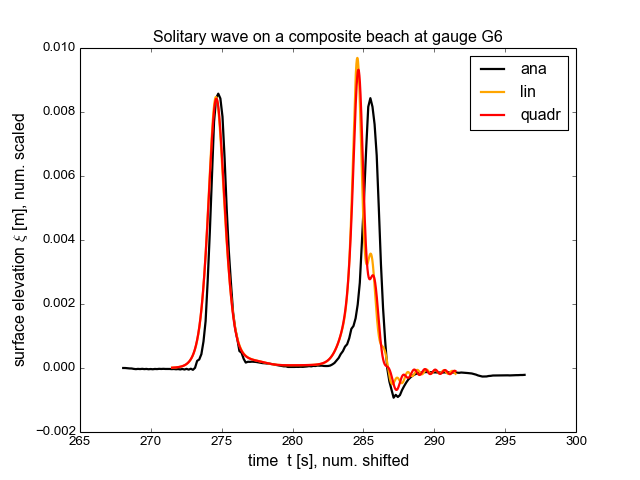
\includegraphics[width=0.48\textwidth]{compositebeach_ana_G6_nh_Nnh12}
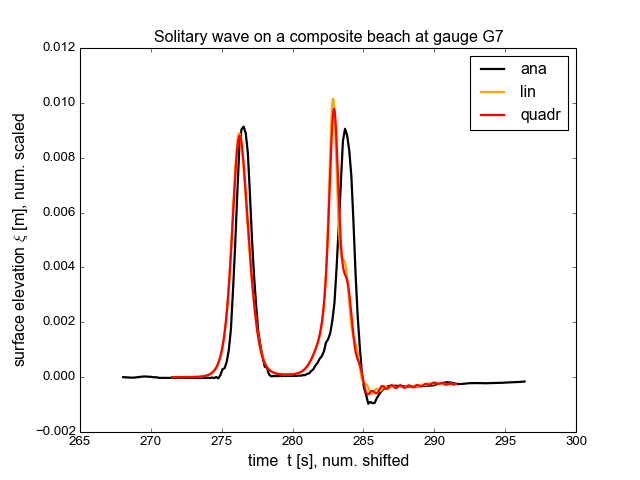
\includegraphics[width=0.48\textwidth]{compositebeach_ana_G7_nh_Nnh12}
\end{minipage} \\
\begin{minipage}{\textwidth}
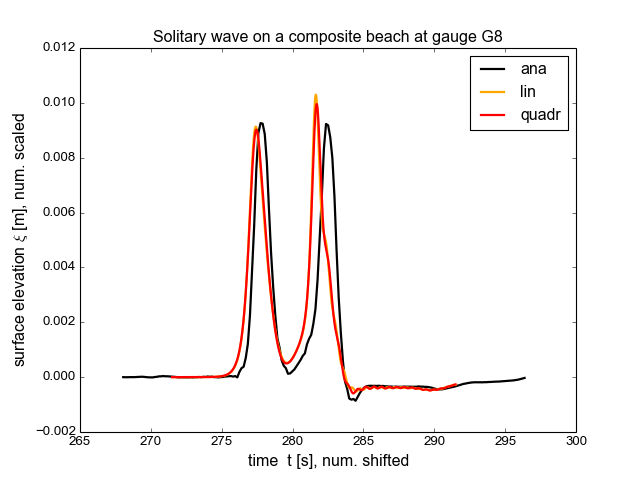
\includegraphics[width=0.48\textwidth]{compositebeach_ana_G8_nh_Nnh12}
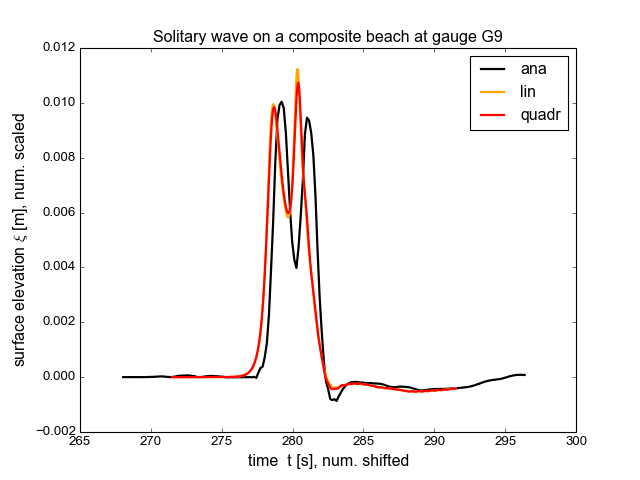
\includegraphics[width=0.48\textwidth]{compositebeach_ana_G9_nh_Nnh12}
\end{minipage} \\
\begin{minipage}{\textwidth}
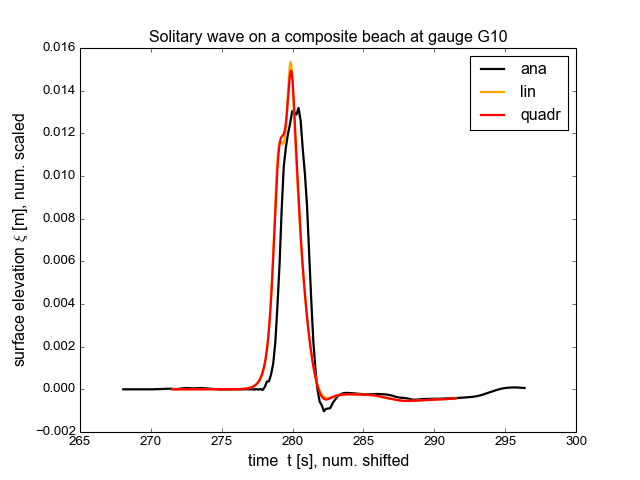
\includegraphics[width=0.48\textwidth]{compositebeach_ana_G10_nh_Nnh12}
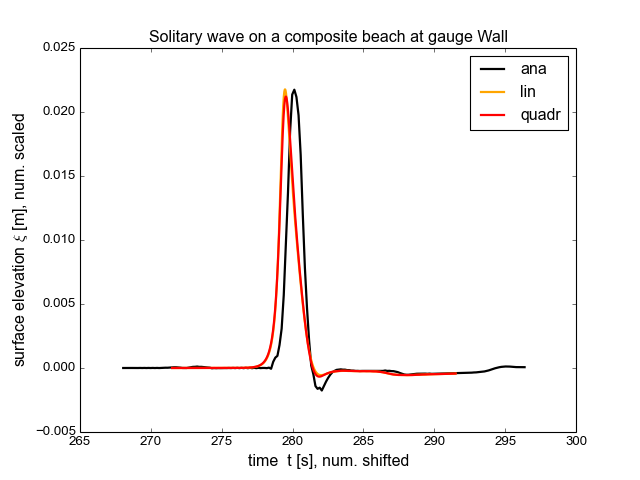
\includegraphics[width=0.48\textwidth]{compositebeach_ana_Wall_nh_Nnh12}
\end{minipage}
\caption{Comparison of the analytical (black) sea surface height of the
solitary wave with the simulation results of the \nh\ model in its \nh\ version using the linear (yellow) and the quadratic vertical pressure profile (red)}
\label{fig:nh_compositebeach_ana_nh_Nnh12}
\end{figure}

\begin{figure}[htbp]
\begin{minipage}{\textwidth}
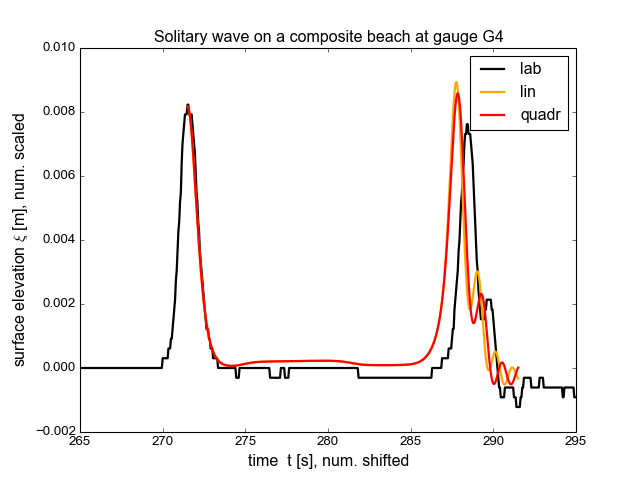
\includegraphics[width=0.48\textwidth]{compositebeach_lab_G4_nh_Nnh12}
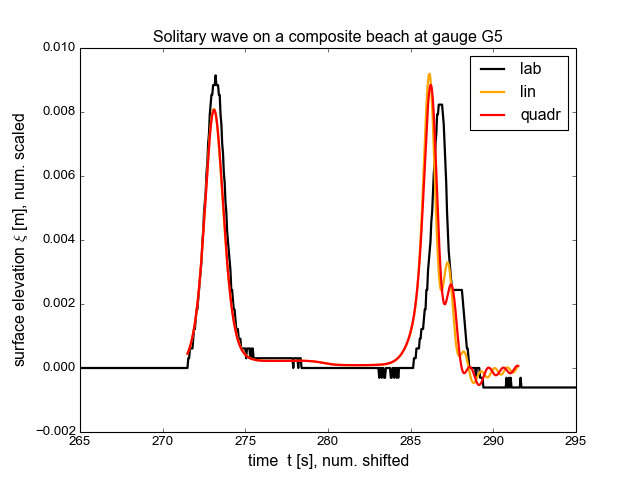
\includegraphics[width=0.48\textwidth]{compositebeach_lab_G5_nh_Nnh12}
\end{minipage} \\
\begin{minipage}{\textwidth}
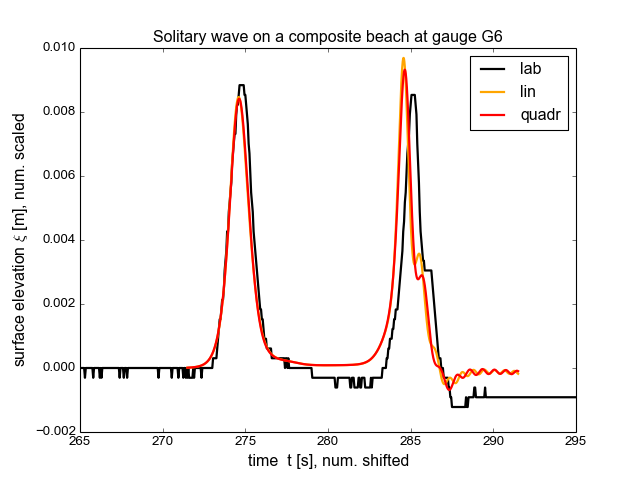
\includegraphics[width=0.48\textwidth]{compositebeach_lab_G6_nh_Nnh12}
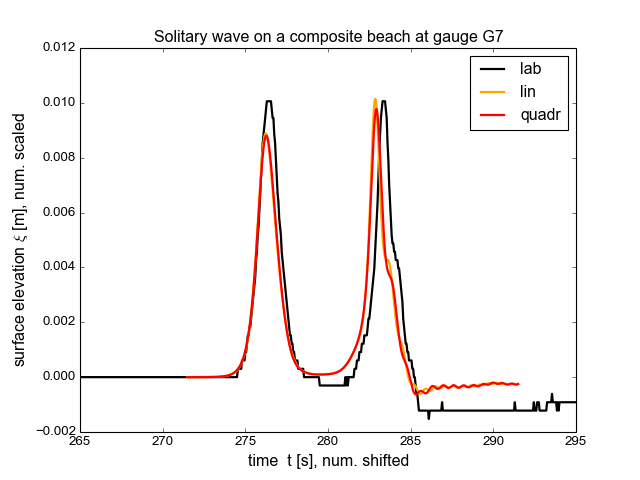
\includegraphics[width=0.48\textwidth]{compositebeach_lab_G7_nh_Nnh12}
\end{minipage} \\
\begin{minipage}{\textwidth}
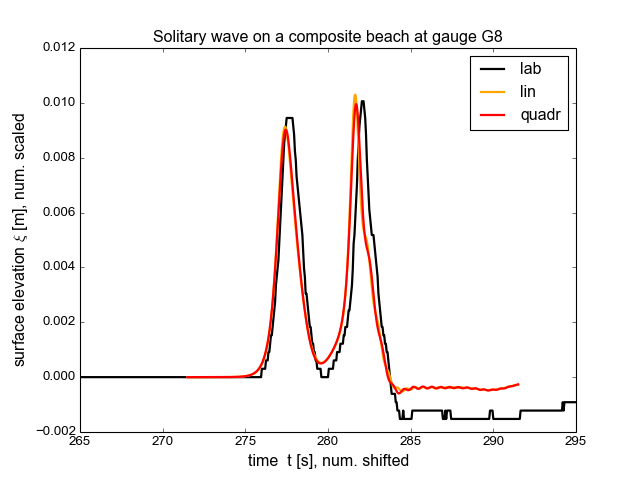
\includegraphics[width=0.48\textwidth]{compositebeach_lab_G8_nh_Nnh12}
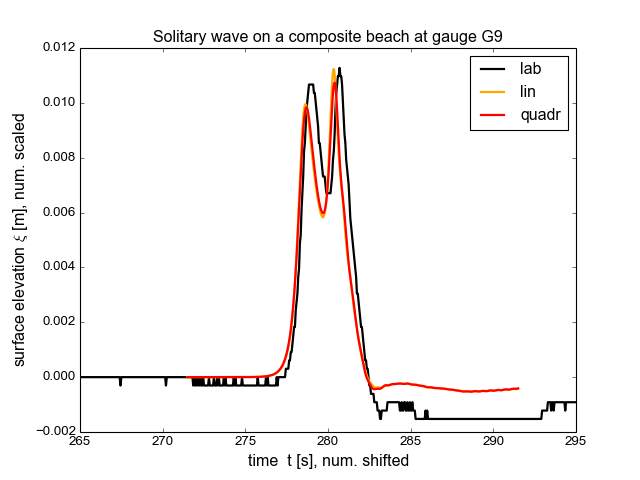
\includegraphics[width=0.48\textwidth]{compositebeach_lab_G9_nh_Nnh12}
\end{minipage} \\
\begin{minipage}{0.48\textwidth}
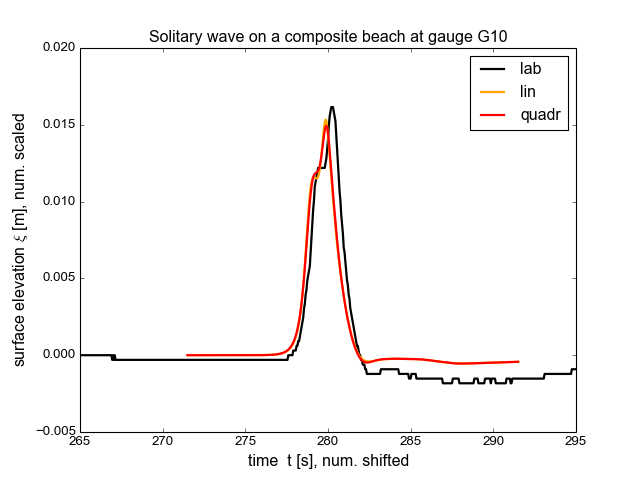
\includegraphics[width=\textwidth]{compositebeach_lab_G10_nh_Nnh12}
\end{minipage} 
\begin{minipage}{0.45\textwidth}
\begin{tabular}{lll}
\textbf{Data} & \textbf{Runup} & \textbf{R / d} \\
              & \textbf{R [cm]} &  \\
\toprule
Exp.  &  2.74   &  0.13 \\
Model lin.&  2.18   &  0.10 \\
Model quadr.&  2.12   &  0.097 \\
\end{tabular}
\end{minipage}
\caption{Comparison of the experimental (black) sea surface height of the
solitary wave with the simulation results of the \nh\ model in its \nh\ version using the linear (yellow) and the quadratic vertical pressure profile (red). The model runup is also scaled with 0.75.}
\label{fig:nh_compositebeach_lab_nh_Nnh12}
\end{figure}

%!TEX root = paper.tex
\subsection{Nonlinear shoaling wave over submerged bar}
In this laboratory experiment an incident sin wave travels over a trapezoidal underwater obstacle and the surface elevations of the non-breaking wave are measured at several gauges spread along the obstacle.
This experiment conducted in different versions by \cite{BejiBattjes.1993} and \cite{BejiBattjes.1994}, \cite{Dingemans.1994} (more cases, here only case A considered), and by Luth et al. (1994) (cited in \cite{Dingemans.1994}, but I do not have access to the report). 
In this experiments, gauges and setups were different (see tables \ref{tab:bejibattjes_gauges_SZ} -- \ref{tab:bejibattjes_gauges_BB1994} and figures \ref{fig:bejibattjes_setup_SZ} -- \ref{fig:bejibattjes_setup_BB1994}).

The setup is as described in \cite{StellingZijlema.2003}, and M. Zijlema provided the data. According to the gauges, this should be the data described in \cite{Dingemans.1994, StellingZijlema.2003} as the data from Luth et al. (1994), but scaled (divided) by a factor of 2. 

The initial condition is the unperturbed state. The boundary condition is described as in incident wave at the left boundary of the computational domain, where the surface elevation is set to $\xi=a \text{sin}\left(\frac{2\pi t}{T}\right)$ with period $T=2.02 \,$s and amplitude $a=1.0\,$cm.
We impose reflecting boundary conditions at the boundary in x-direction and periodic boundary conditions in y-direction. For the setup see figure \ref{fig:bejibattjes_setup_SZ}. The computational domain is enlarged to 40m to ensure no reflecting waves disturbing the solution during the simulation time of 40s.

Note: No boundary conditions are specified for w and q at the moment, computations which set them to zero are running. This hopefully explains the wrong behavior. 


\begin{table}[htbp]
\begin{tabular}{lllllllll}
\textbf{gauge} & G4 & G5 & G6 & G7 & G8 & G9 & G10 & G11 \\
\toprule
\textbf{x [m]} & 10.5 & 12.5 & 13.5 & 14.5 & 15.7 & 17.3 & 19.9 & 21.0 \\
\bottomrule
\end{tabular}
\caption{Locations of gauges used in \cite{StellingZijlema.2003}}
\label{tab:bejibattjes_gauges_SZ}
\end{table}

\begin{table}[htbp]
\begin{tabular}{lllllllll}
\textbf{gauge} & 1 & 2 & 3 & 4 & 5 & 6 & 7 & 8 \\
\toprule
\textbf{x [m]} & 6.0 & 11.0 & 12.0 & 13.0 & 14.0 & 15.0 & 16.0 & 17.0 \\
\bottomrule
\end{tabular}
\caption{Locations of gauges used in \cite{BejiBattjes.1993}}
\label{tab:bejibattjes_gauges_BB1993}
\end{table}

\begin{table}[htbp]
\begin{tabular}{llllllll}
\textbf{gauge} & 1 & 2 & 3 & 4 & 5 & 6 & 7 \\
\toprule
\textbf{x [m]} & 6 & 10.8 & 12.8 & 13.8 & 14.8 & 16.0 & 17.6 \\
\bottomrule
\end{tabular}
\caption{Locations of gauges used in \cite{BejiBattjes.1994}}
\label{tab:bejibattjes_gauges_BB1994}
\end{table}

\begin{figure}[htbp]
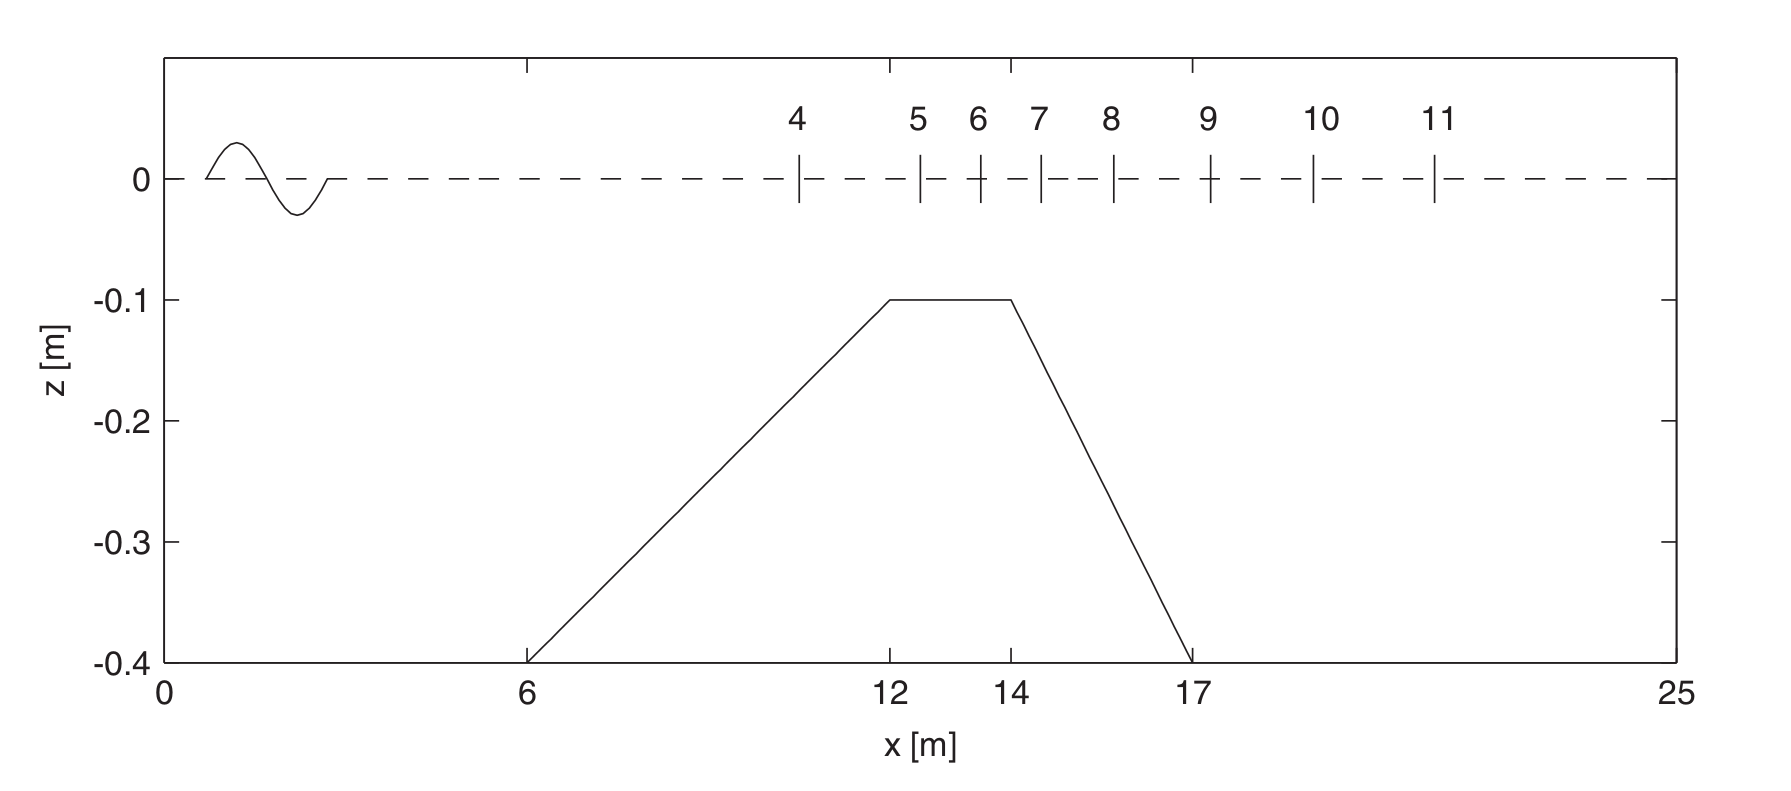
\includegraphics[width=\textwidth]{bejibattjes_setup_SZ}
\caption{Setup of the experiment of Beji and Battjes according to \cite{StellingZijlema.2003}}
\label{fig:bejibattjes_setup_SZ}
\end{figure}

\begin{figure}[htbp]
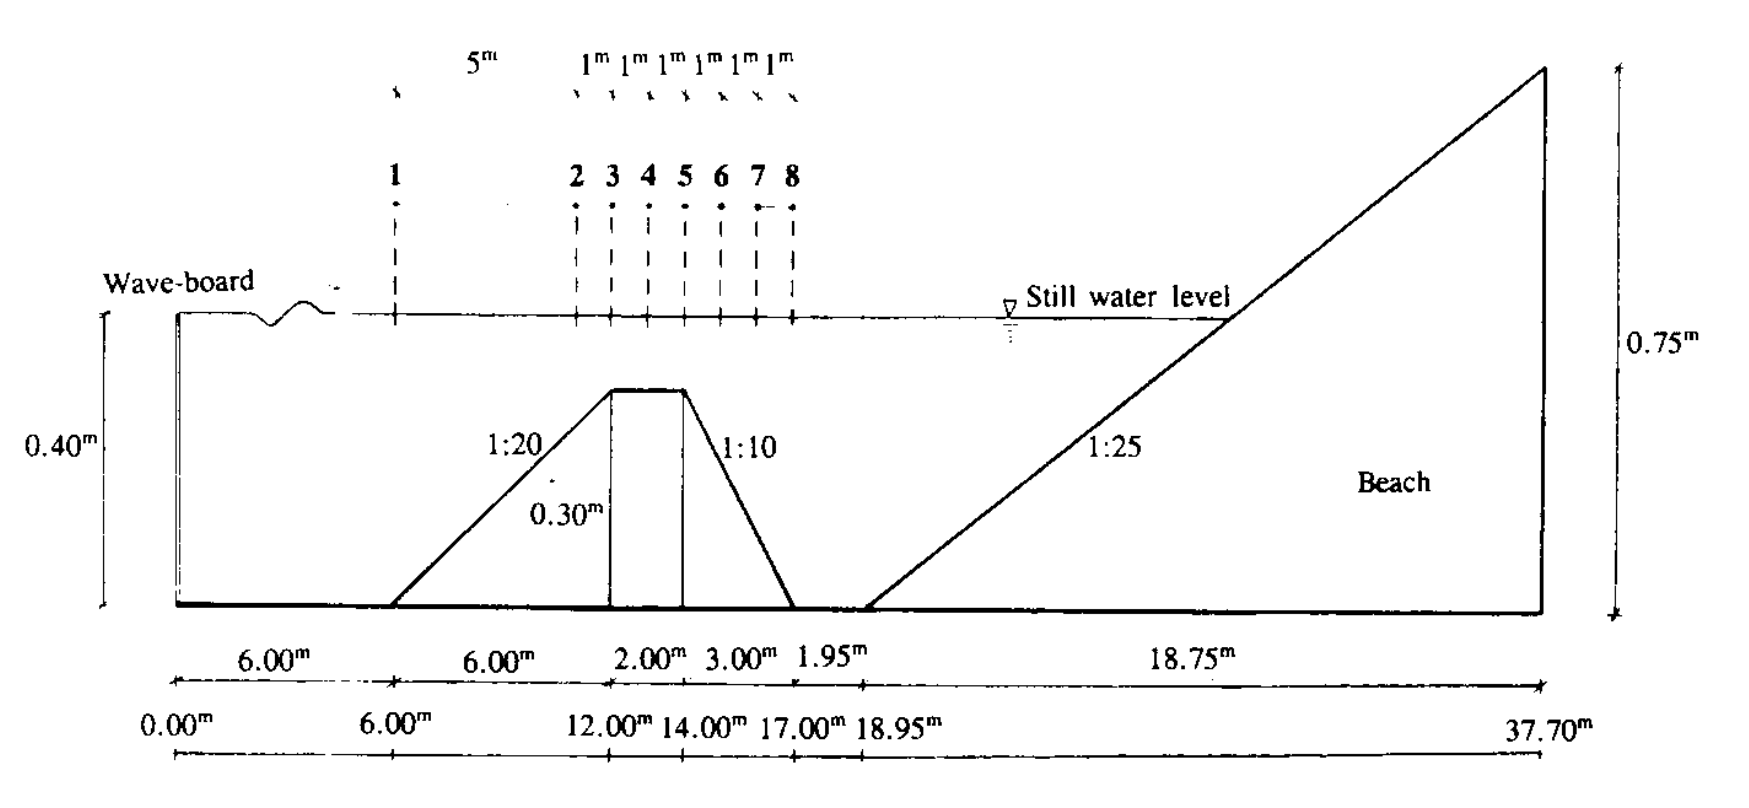
\includegraphics[width=\textwidth]{bejibattjes_setup_BB1993}
\caption{Setup of the experiment of Beji and Battjes according to \cite{BejiBattjes.1993}}
\label{fig:bejibattjes_setup_BB1993}
\end{figure}

\begin{figure}[htbp]
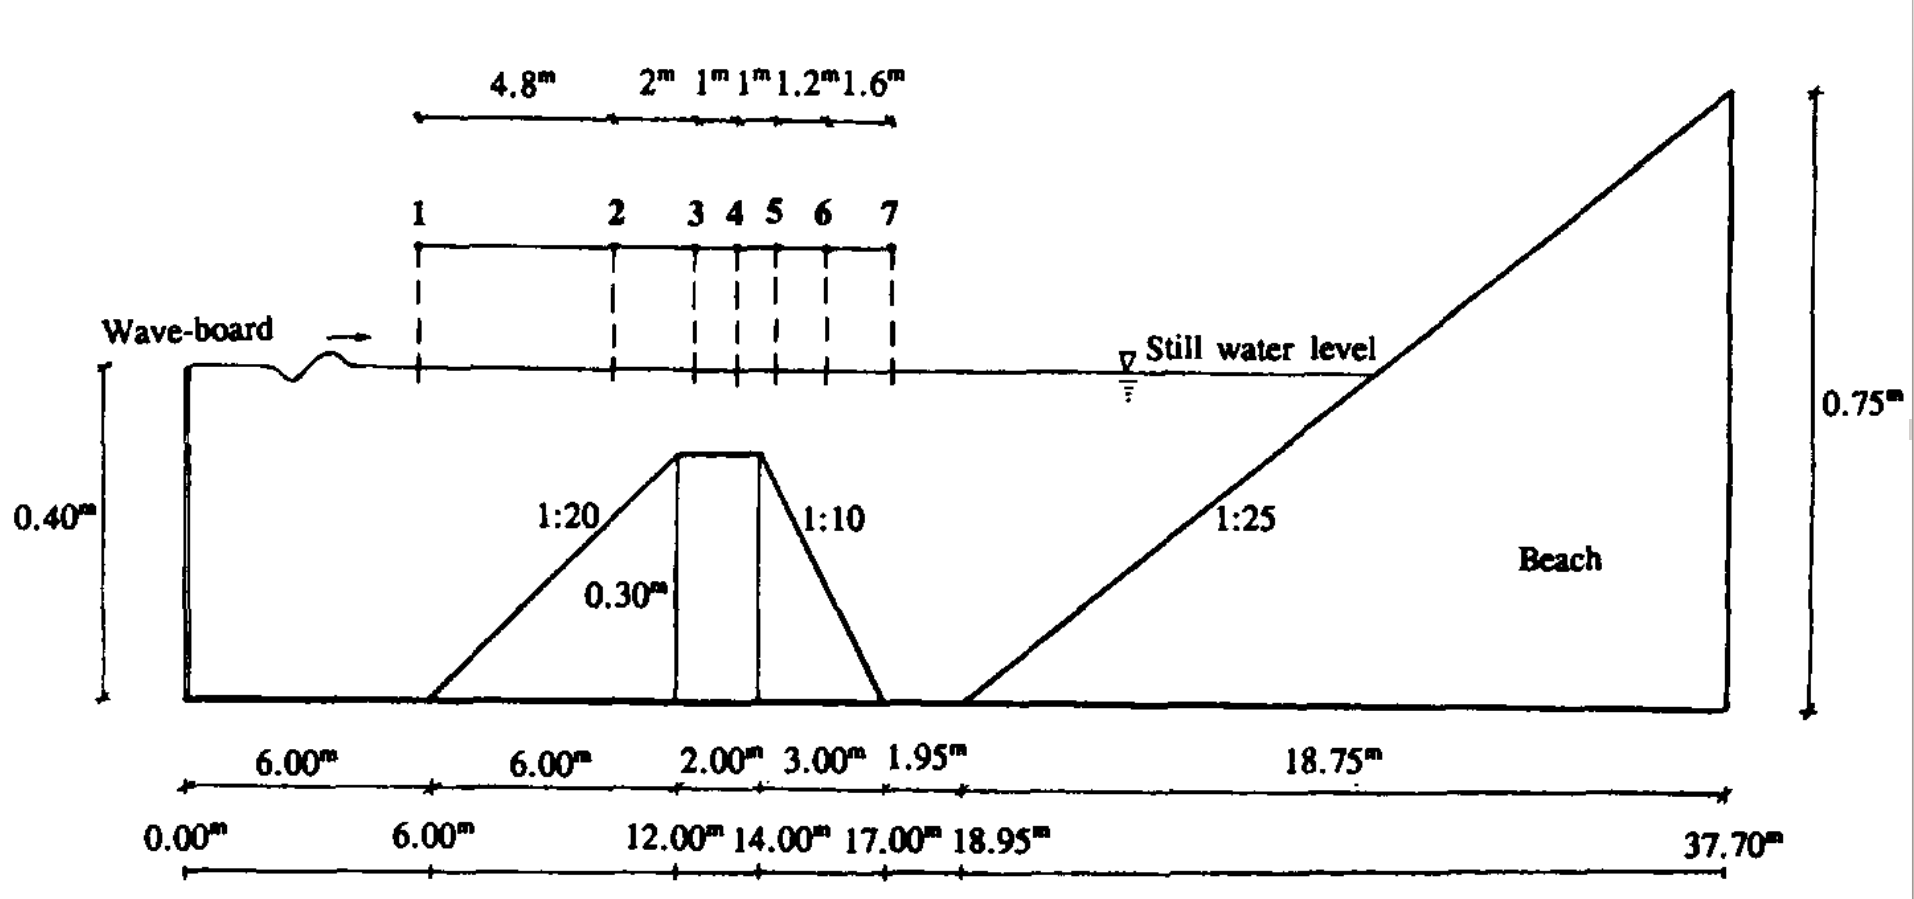
\includegraphics[width=\textwidth]{bejibattjes_setup_BB1994}
\caption{Setup of the experiment of Beji and Battjes according to \cite{BejiBattjes.1994}}
\label{fig:bejibattjes_setup_BB1994}
\end{figure}

\subsubsection{Results of \nh\ model}
The model results can be found in figure \eqref{fig:nh_bejjibattjes_nh}.
The results are shifted in time by 4.5s to match the laboratory data at gauge 10 in phase after 20s.

\begin{figure}[htbp]
\begin{minipage}{\textwidth}
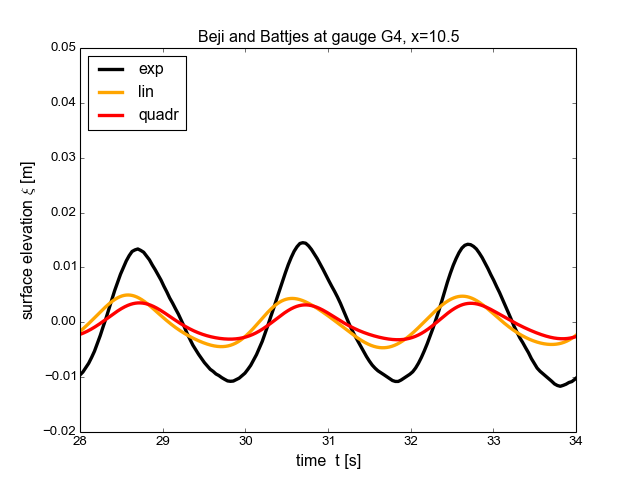
\includegraphics[width=0.48\textwidth]{BejiBattjes_nh_x=loc_4}
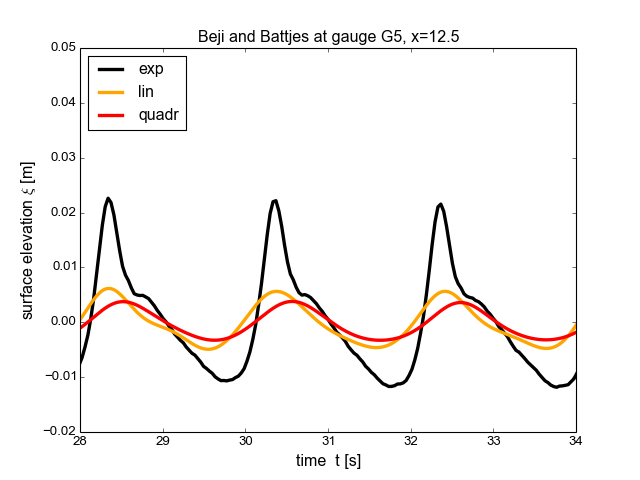
\includegraphics[width=0.48\textwidth]{BejiBattjes_nh_x=loc_5}
\end{minipage} \\
\begin{minipage}{\textwidth}
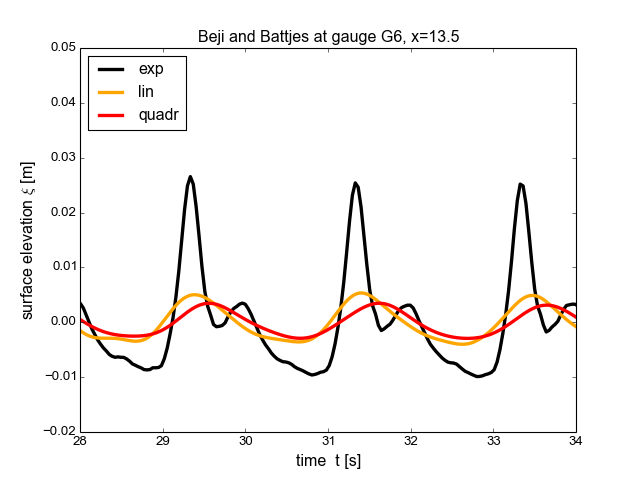
\includegraphics[width=0.48\textwidth]{BejiBattjes_nh_x=loc_6}
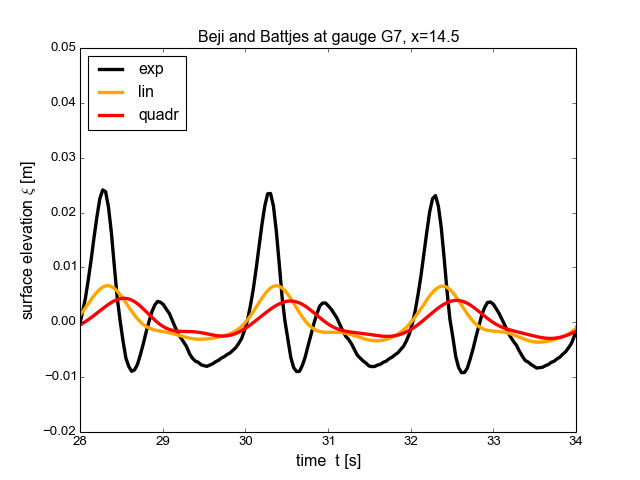
\includegraphics[width=0.48\textwidth]{BejiBattjes_nh_x=loc_7}
\end{minipage} \\
\begin{minipage}{\textwidth}
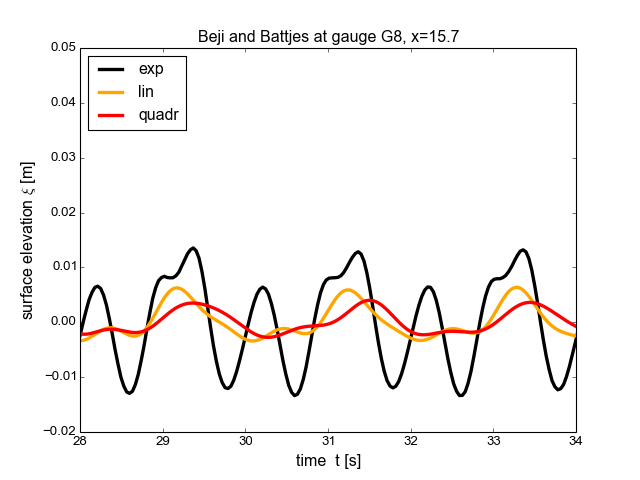
\includegraphics[width=0.48\textwidth]{BejiBattjes_nh_x=loc_8}
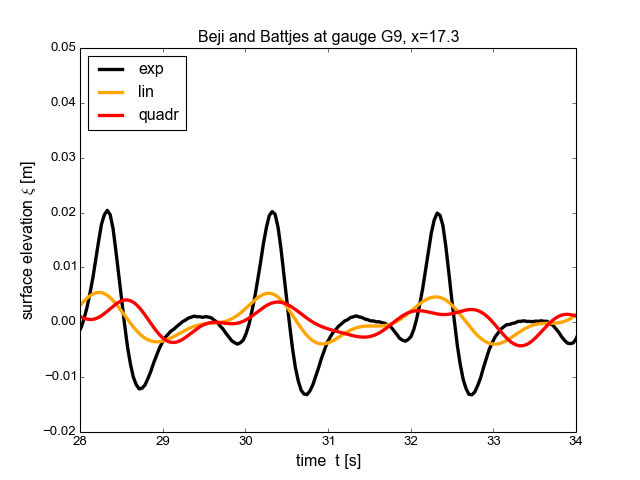
\includegraphics[width=0.48\textwidth]{BejiBattjes_nh_x=loc_9}
\end{minipage} \\
\begin{minipage}{\textwidth}
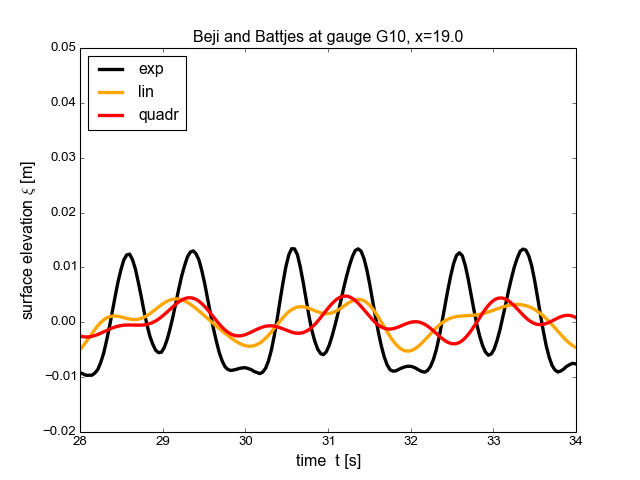
\includegraphics[width=0.48\textwidth]{BejiBattjes_nh_x=loc_10}
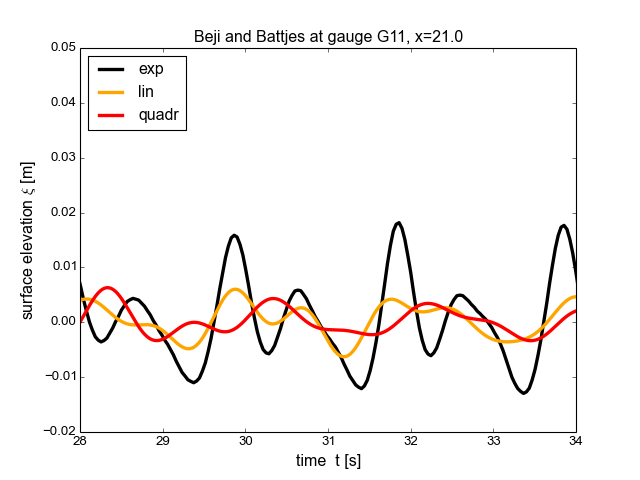
\includegraphics[width=0.48\textwidth]{BejiBattjes_nh_x=loc_11}
\end{minipage}
\caption{Comparison of the laboratory (black) sea surface height at gauges with the simulation results of the \nh\ model with linear pressure profile (yellow) and quadratic pressure profile (red)}
\label{fig:nh_bejjibattjes_nh}
\end{figure}

\begin{flushleft}
    \bibliographystyle{abbrv}
    \bibliography{references}
    \addcontentsline{toc}{section}{References}
\end{flushleft}

\end{document}
